% Options for packages loaded elsewhere
\PassOptionsToPackage{unicode}{hyperref}
\PassOptionsToPackage{hyphens}{url}
%
\documentclass[
]{article}
\title{Model ThreeMe Tunisia}
\usepackage{etoolbox}
\makeatletter
\providecommand{\subtitle}[1]{% add subtitle to \maketitle
  \apptocmd{\@title}{\par {\large #1 \par}}{}{}
}
\makeatother
\subtitle{Macroeconomic impacts of National Low-Carbon Strategy for a
little country in development : the case of Tunisia}
\author{Lucia SEQUEIRA - Bijan VALILOU - Jin WANG}
\date{January 2022}

\usepackage{amsmath,amssymb}
\usepackage{lmodern}
\usepackage{iftex}
\ifPDFTeX
  \usepackage[T1]{fontenc}
  \usepackage[utf8]{inputenc}
  \usepackage{textcomp} % provide euro and other symbols
\else % if luatex or xetex
  \usepackage{unicode-math}
  \defaultfontfeatures{Scale=MatchLowercase}
  \defaultfontfeatures[\rmfamily]{Ligatures=TeX,Scale=1}
\fi
% Use upquote if available, for straight quotes in verbatim environments
\IfFileExists{upquote.sty}{\usepackage{upquote}}{}
\IfFileExists{microtype.sty}{% use microtype if available
  \usepackage[]{microtype}
  \UseMicrotypeSet[protrusion]{basicmath} % disable protrusion for tt fonts
}{}
\makeatletter
\@ifundefined{KOMAClassName}{% if non-KOMA class
  \IfFileExists{parskip.sty}{%
    \usepackage{parskip}
  }{% else
    \setlength{\parindent}{0pt}
    \setlength{\parskip}{6pt plus 2pt minus 1pt}}
}{% if KOMA class
  \KOMAoptions{parskip=half}}
\makeatother
\usepackage{xcolor}
\IfFileExists{xurl.sty}{\usepackage{xurl}}{} % add URL line breaks if available
\IfFileExists{bookmark.sty}{\usepackage{bookmark}}{\usepackage{hyperref}}
\hypersetup{
  pdftitle={Model ThreeMe Tunisia},
  pdfauthor={Lucia SEQUEIRA - Bijan VALILOU - Jin WANG},
  hidelinks,
  pdfcreator={LaTeX via pandoc}}
\urlstyle{same} % disable monospaced font for URLs
\usepackage[margin=1in]{geometry}
\usepackage{graphicx}
\makeatletter
\def\maxwidth{\ifdim\Gin@nat@width>\linewidth\linewidth\else\Gin@nat@width\fi}
\def\maxheight{\ifdim\Gin@nat@height>\textheight\textheight\else\Gin@nat@height\fi}
\makeatother
% Scale images if necessary, so that they will not overflow the page
% margins by default, and it is still possible to overwrite the defaults
% using explicit options in \includegraphics[width, height, ...]{}
\setkeys{Gin}{width=\maxwidth,height=\maxheight,keepaspectratio}
% Set default figure placement to htbp
\makeatletter
\def\fps@figure{htbp}
\makeatother
\setlength{\emergencystretch}{3em} % prevent overfull lines
\providecommand{\tightlist}{%
  \setlength{\itemsep}{0pt}\setlength{\parskip}{0pt}}
\setcounter{secnumdepth}{5}
\usepackage{fancyhdr}
\pagestyle{fancy}
\fancyfoot[CO,CE]{Modèle ThreeMe Tunisie}
\fancyfoot[LE,RO]{\thepage}
\usepackage{booktabs}
\usepackage{longtable}
\usepackage{array}
\usepackage{multirow}
\usepackage{wrapfig}
\usepackage{float}
\usepackage{colortbl}
\usepackage{pdflscape}
\usepackage{tabu}
\usepackage{threeparttable}
\usepackage{threeparttablex}
\usepackage[normalem]{ulem}
\usepackage{makecell}
\usepackage{xcolor}
\ifLuaTeX
  \usepackage{selnolig}  % disable illegal ligatures
\fi
\usepackage[]{biblatex}
\addbibresource{references.bib}

\begin{document}
\maketitle

{
\setcounter{tocdepth}{2}
\tableofcontents
}
\newpage

\hypertarget{introduction}{%
\section{Introduction}\label{introduction}}

\hypertarget{literature-review}{%
\section{Literature review}\label{literature-review}}

\hypertarget{energy-and-economy-framework-in-tunisia-jin}{%
\subsection{Energy and economy framework in Tunisia
(Jin)}\label{energy-and-economy-framework-in-tunisia-jin}}

Tunisia is one of the northernmost countries in Africa, ranked the most
competitive economy in Africa by World Economy Forum in 2009
\autocite{tunisia2022}. The local economy is largely oriented towards
services, which account for 43\% of GDP in 2019
\autocite{worldbank2020}, including the booming IT and tourism
industries. Agriculture is another key sector of the Tunisian economy,
representing 10.4\% of the GDP and employing 12.7\% of the working
population \autocite{worldbank2020}. Thanks to technical progress of
agricultural sector, Tunisia is one of the most productive countries in
Africa. Tunisia's industry represents 22.7\% of GDP and employs 32.5\%
of the working population in 2020 \autocite{bnpparibas}. The industrial
sectors are mainly export oriented especially for manufacturing, Europe
is the destination for more than 75\% of Tunisia's exports
\autocite{worldbank2020}.

Since the Jasmine Revolution on 2011, Tunisia economy has been suffered
from the extended recession. The sanitary crisis on 2020 has worsened
the already precarious situation. Actually, even before COVID-19
Tunisia's capacity for economic resilience had been drained by years of
indecisive public policy-making and growing protectionism
\autocite{worldbank}. In early September 2020, the Tunisian parliament
finally reversed a government of Tenchnocrats in an attempt to remedy
the country's economic situation \autocite{bnpparibas}.

Along with the sluggish economy is the huge energy deficit in Tunisia.
\textcite{irena2021} reported that energy deficit (50\% in 2019) has
existed in Tunisia over the past two decades, mainly because of the
increasing consumption but with the stagnated even declined domestic
production in recent years. \textcite{giz} reported that Tunisia depends
for 60\% on energy imports, and this number is continuously raising. The
energy transition project proclaimed in 2014 aims to reduce energy needs
by 34\% by 2030, lower subsidies and establish incentive mechanisms
favoring profitable and climate friendly investments. However, the
challenging is the lack of reliable institutional mechanisms and
motivation for enterprises to participate, accompanied with a poorly
established service market and weak transmission of knowledge to
citizens, especially outside urban area.

\hypertarget{climate-policy}{%
\subsection{Climate policy}\label{climate-policy}}

\hypertarget{carbon-tax-jin}{%
\subsubsection{Carbon tax (Jin)}\label{carbon-tax-jin}}

\hypertarget{energetic-subsidy-bee}{%
\subsubsection{Energetic subsidy (Bee)}\label{energetic-subsidy-bee}}

Subsidies are defined by \textcite{demoor1997} as \emph{`any measure
that keeps prices for consumers below the market level or keeps prices
for producers above the market level or that reduces costs for consumers
and producers by giving direct or indirect support'}. Energy subsidies
are a common policy. Their amount is estimated at \$4.7 trillion in 2015
as pointed out \textcite{coady2019}, which is equivalent to 6.3 percent
of Gross Domestic Product . Energy subsidies fluctuate depending on the
price of the energy products. From the database of the International
Energy Agency, we can notice that the fossil fuel subsidies have
\href{https://www.iea.org/topics/energy-subsidies}{fallen by 42 percent
between 2019 and 2020} due to the drop of fuel prices.

The energy subsidies are very present in the Middle East, North Africa,
Afghanistan and Pakistan region (MENAP). According to
\textcite{coady2019}, MENAP is the fourth region in absolute terms,
which subsidized the most energy in 2015. Nevertheless, in relative
terms, MENAP is the second, if we take into account the percent of its
GDP. The prevalence of energy subsidies in MENAP can be explained by
post-par period. \textcite{verme2017} explain that theses energy
subsidies were introduced in Middle East and North Africa region (MENA)
in order to stabilize prices after the decolonization. These
stabilization mechanisms became a social protection system.

\hypertarget{recycle-of-gouvernment-income-for-tax-lucia}{%
\subsubsection{Recycle of gouvernment income for tax
(Lucia)}\label{recycle-of-gouvernment-income-for-tax-lucia}}

\hypertarget{methodology}{%
\section{Methodology}\label{methodology}}

\hypertarget{threeme-model-bee}{%
\subsection{ThreeME model (Bee)}\label{threeme-model-bee}}

\hypertarget{a-neo-keynesian-computable-general-equilibrium-model}{%
\subsubsection{A neo-Keynesian Computable General Equilibrium
model}\label{a-neo-keynesian-computable-general-equilibrium-model}}

\hypertarget{threeme-model-tunisia-adaptation-for-a-little-country-in-development}{%
\subsubsection{ThreeMe model Tunisia : Adaptation for a little country
in
development}\label{threeme-model-tunisia-adaptation-for-a-little-country-in-development}}

\hypertarget{description-of-scenario}{%
\subsection{Description of scenario}\label{description-of-scenario}}

with/without redistribution

\hypertarget{tax-carbone}{%
\subsubsection{Tax carbone}\label{tax-carbone}}

Avant 2030, le niveau de la TC est calculé de façon a couvrir 100\% des
besoins du FTE Il passe de 1.1 à 9 DT/tCO2 Après 2030, la trajectoire de
la TC est définie de façon à atteindre les objectifs de réduction
d'émission à 2050 D'après les hypothèse des substitutions retenues dans
ThreeME, l'atteinte d'un factor 5 en 2050 par rapport au niveau de 2020
nécessite une hause régulière de 9 DT/tCO2 à 372 DT/ tCO2. En plus de la
TC des signaux prix ont été introduits afin d'atteindre les objectifs de
consommations d'énergie par source

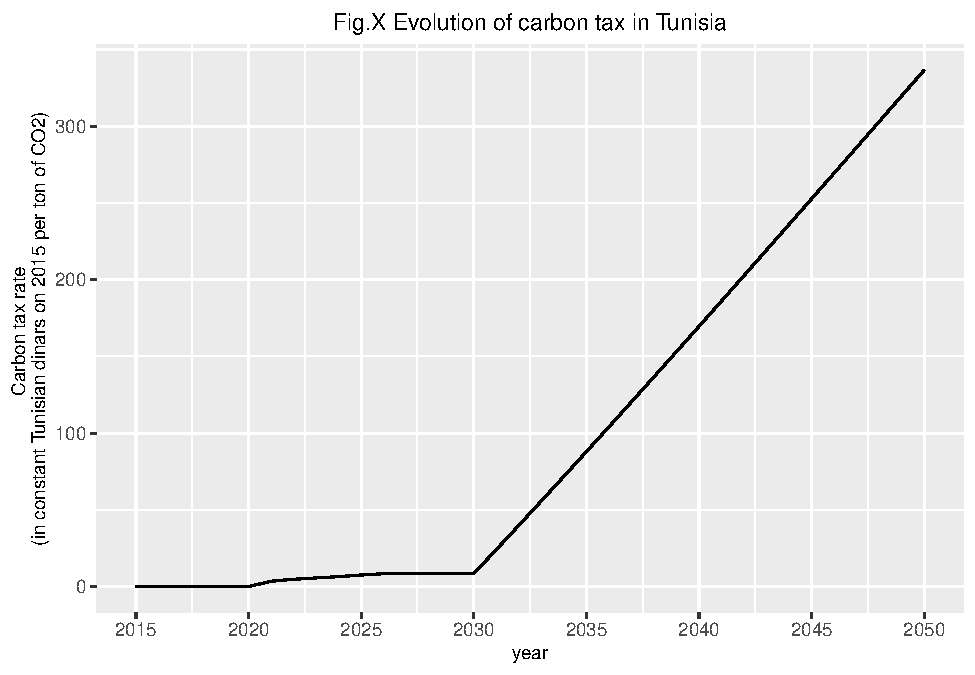
\includegraphics{Modele-ThreeMe-Tunisie_Sequeira_Valilou_Wang_files/figure-latex/unnamed-chunk-6-1.pdf}

\hypertarget{energy-subsidy}{%
\subsubsection{Energy subsidy}\label{energy-subsidy}}

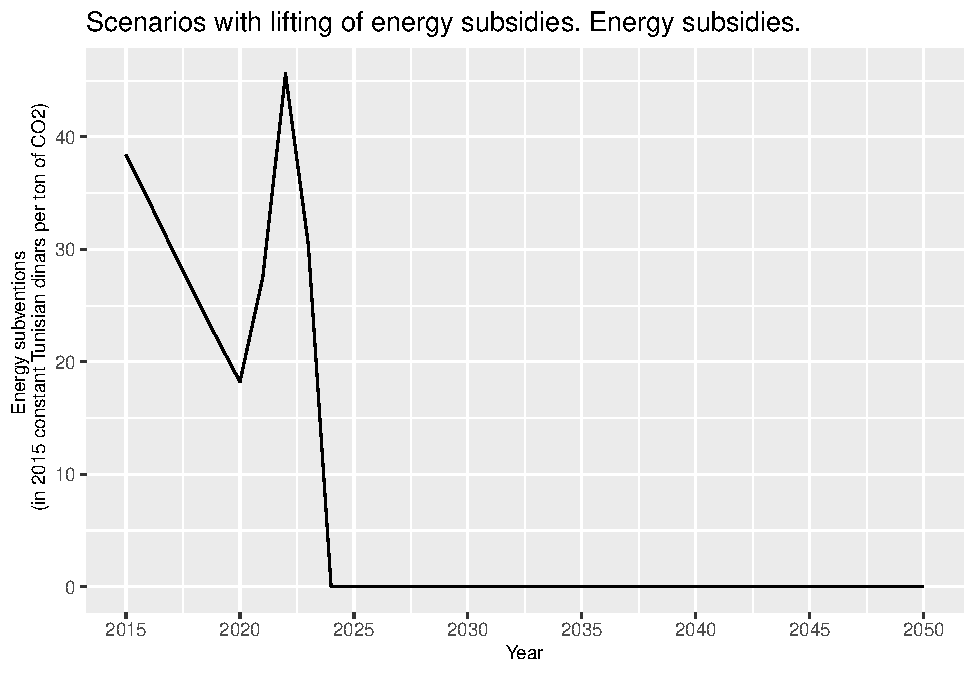
\includegraphics{Modele-ThreeMe-Tunisie_Sequeira_Valilou_Wang_files/figure-latex/unnamed-chunk-7-1.pdf}

\hypertarget{enr}{%
\subsubsection{ENR}\label{enr}}

\hypertarget{snbc}{%
\subsubsection{SNBC}\label{snbc}}

\hypertarget{choice-of-evaluation-indicators}{%
\subsection{Choice of evaluation
indicators}\label{choice-of-evaluation-indicators}}

\hypertarget{data-structure}{%
\subsubsection{Data structure}\label{data-structure}}

All the indicators used in the analysis are in exact hat algebra,
meaning the proportional variation to Baseline scenario. time scale of
data key indicator: two dimensions economy and environnement

\hypertarget{kaya-identity-jin}{%
\subsubsection{Kaya identity (Jin)}\label{kaya-identity-jin}}

The Kaya identity, firstly proposed by \autocite{kaya1989}, is an
identity where the total emission of carbon dioxide can be explained by
four product driving forces as population, Gross Domestic Product (GDP)
per capita, enerny intensity over GDP and carbon intensity over energy
consumption \autocite{kayaide2021}. It is expressed in the form:

\[ C = POP \cdot \frac{GDP}{POP} \cdot \frac{TEC}{GDP} \cdot \frac{C}{TEC} \tag{1}\]

where:

\begin{itemize}
\tightlist
\item
  POP is global population;
\item
  GDP is gross domestic product;
\item
  TEC is total energy consumption;
\item
  C is total emission of carbon dioxide;
\end{itemize}

And:

\begin{itemize}
\tightlist
\item
  GDP/POP is GDP per capita describing the economical activities within
  a period;
\item
  TEC/GDP is energy intensity;
\item
  C/TEC is carbon intensity;
\end{itemize}

In this study, we introduced an extension of Kaya identity to explain
how different driving forces influenced the total emission for different
scenarios. Firstly, a extended Kaya identity is used to analysis
CO\textsubscript{2} emission with the aggregated factors, then we couple
with Logarithmic Mean Divisia Index (LMDI) method to decomposite
CO\textsubscript{2} emission at the sectorial level.

We modified the function of Kaya identity mentioned above to adapt our
model assumption, where we integrated a new driving force, named economy
structure, to decomposite emissions driving force at sectorial level.
The five economic sectors considered in ThreeME Tunisia model are:
Industry and Agriculture, Service, Transportation, Energy Transformation
and Electricity. However, we did not take population into consideration
because its increasing rate remains still over time for all our
scenarios and is considered as an exogenous variable in ThreeME model.

Therefore, the CO\textsubscript{2} emission can be written as:

\[  C_{tot} = \Sigma C_{i} = \Sigma( VA \cdot \frac{VA_{i}}{VA} \cdot \frac{EC_{i}}{VA_{i}} \cdot \frac{CE_{i}}{EC_{i}} )=  \Sigma( V \cdot S_{i} \cdot E_{i} \cdot I_{i}) \tag{2}\]
where C\textsubscript{tot} is overall CO\textsubscript{2} emission,
C\textsubscript{i} is CO\textsubscript{2} emission of economic sector i,
VA is total added value, VA\textsubscript{i} is added value of sector i,
EC\textsubscript{i} is total energy consumption by sector i,
CE\textsubscript{i} is CO\textsubscript{2} emission arising from sector
i. According to equation 8, total CO\textsubscript{2} emission can be
explained by four driving forces, including one aggregated indicator,
overall economic activities V, and three sectorial indicators, share of
total added value of sector i S\textsubscript{i}, energy intensity over
added value of sector i E\textsubscript{i} and carbon intensity over
energy consumption of sector i I\textsubscript{i}. Especially,
S\textsubscript{i} can be interpreted as economy structure of Tunisia,
\textcite{grubb2015} and \textcite{kanitkar2015} found that for a
developing country, this term could be a key variable determining the
future emissions pathway.

The effects of driving forces can be expressed in two ways:
multiplicative and additive form, where multiplicative deviation
\(D_{tot}\) is the ratio of total CO\textsubscript{2} emission between
policy scenario and baseline scenario (equation 3), and additive
deviation \(\Delta C_{tot}\) is the difference of total
CO\textsubscript{2} emission (equation 4). The two expressions are shown
below:

\[ D_{tot} =\frac{C_{2}}{C_{0}} = \Pi(\frac{V_{2}}{V_{0}} \cdot \frac{S_{2,i}}{S_{0,i}} \cdot \frac{E_{2,i}}{E_{0,i}}  \cdot \frac{I_{2,i}}{I_{0,i}}) = D_{V}  \cdot  D_{S} \cdot D_{E} \cdot D_{I} = D_{V}  \cdot \Pi ( D_{S_{i}} \cdot D_{E_{i}} \cdot D_{I_{i}}) \tag{3}\]

\[ \Delta C_{tot} = C_{2} - C_{0} = \Delta C_{V} + \Delta C_{S} + \Delta C_{E} + \Delta C_{I} = \Delta C_{V} + \Sigma( \Delta C_{S_{i}} + \Delta C_{E_{i}} + \Delta C_{I_{i}}) \tag{4}\]
where subscript \(tot\) represents overall change of emission, subscript
0 and 2 mean baseline scenario and policy scenario respectively. Hence
we obtain the index \(D_{V}\), \(D_{S}\), \(D_{E}\) and \(D_{I}\),
meaning the deviation of emissions due to change of overall economic
activities, economy structure, energy intensity and carbon intensity,
while \(\Delta C_{V}\), \(\Delta C_{S}\), \(\Delta C_{E}\) and
\(\Delta C_{I}\) depict the difference of emissions related to change of
driving forces.

Now we expect to identify the effect of each driving force at a
sectorial level, to do this, we used a LMDI method proposed by
\textcite{ang1997} and \textcite{ang2005}. For multiplicative form, we
have:

\[ D_{X} = exp ( \Sigma \frac{(C_{2,i}-C_{0,i})/(lnC_{2,i}-lnC_{0,i})}{(C_{2}-C_{0})/(lnC_{2}-lnC_{0})} \cdot ln \frac{X_{2,(i)}}{X_{0,(i)}} ) \tag{11}\]
\[ \Delta C_{X} =  \Sigma (\frac{C_{2,i}-C_{0,i}}{lnC_{2,i}-lnC_{0,i}} \cdot ln\frac{X_{2,(i)}}{X_{0,(i)}}) \tag{12} \]
where \(C_{2}\) is total emission of policy scenario, \(C_{0}\) is total
emission of baseline, \(C_{2,i}\) is emission of policy scenario arising
from sector i, \(C_{0,i}\) is emission of baseline arising from sector
i, \(D_{X}\) and \(\Delta C_{X}\) represent multiplicative and additive
index of driving force \(X\), \(X_{2,(i)}\) is value of driving force
\(X\) of policy scenario for sector i, \(X_{0,(i)}\) is value of driving
force \(X\) of baseline for sector i.

\hypertarget{results-et-discussions}{%
\section{Results et discussions}\label{results-et-discussions}}

\hypertarget{comparasion-of-redistribution-lucia}{%
\subsection{Comparasion of redistribution
(lucia)}\label{comparasion-of-redistribution-lucia}}

\begin{itemize}
\tightlist
\item
  graphique PIB : grandes tendances des scénarii Taxe carbone, Levée des
  subventions énergétiques
\item
  chomage : grandes tendances des scénarii Taxe carbone, Levée des
  subventions énergétiques
\item
  émissions : grandes tendances des scénarii Taxe carbone, Levée des
  subventions énergétiques
\end{itemize}

\hypertarget{carbon-tax-jin-1}{%
\subsection{Carbon tax (jin)}\label{carbon-tax-jin-1}}

As the carbon tax before 2030 stays at a moderate level, the impacts of
this policy are therefore limited, while the significant effects are
observed during the later period from 2030 to 2050 when a much stronger
tax carbon is implemented. The macroeconomic impacts are summarized in
table 1, the results are expressed as percentage deviation from Baseline
scenario.

Generally speaking, the policy of carbon tax with redistribution of
government revenue has a positive impact on Tunisia's economy. Whereas
GDP increases slightly up to 0.13\% with respect to baseline on 2030,
the relatively rapid augmentation is observed from 2030 to 2050. At the
horizon of 2050, it reaches a highest level (+1.93\%) thanks to the
carbon tax policy. In the meantime, social welfare is improved with the
same rhythme as GDP growth, with a higher consumption level (+4.20\%)
and a higher disposable income (+4.17\%) on 2050.

\begin{longtabu} to \linewidth {>{\raggedright}X>{\raggedleft}X>{\raggedleft}X>{\raggedleft}X>{\raggedleft}X>{\raggedleft}X>{\raggedleft}X>{\raggedleft}X}
\caption{\label{tab:unnamed-chunk-8}Macroeconomic impacts of Carbon tax scenario in % deviation to Baseline}\\
\toprule
\textbf{ } & \textbf{2021} & \textbf{2025} & \textbf{2030} & \textbf{2035} & \textbf{2040} & \textbf{2045} & \textbf{2050}\\
\midrule
\endfirsthead
\caption[]{Macroeconomic impacts of Carbon tax scenario in % deviation to Baseline \textit{(continued)}}\\
\toprule
\textbf{ } & \textbf{2021} & \textbf{2025} & \textbf{2030} & \textbf{2035} & \textbf{2040} & \textbf{2045} & \textbf{2050}\\
\midrule
\endhead

\endfoot
\bottomrule
\endlastfoot
\cellcolor{gray!6}{GDP in volume} & \cellcolor{gray!6}{0.03} & \cellcolor{gray!6}{0.11} & \cellcolor{gray!6}{0.13} & \cellcolor{gray!6}{0.97} & \cellcolor{gray!6}{1.56} & \cellcolor{gray!6}{1.87} & \cellcolor{gray!6}{1.93}\\
Household consumption & 0.02 & 0.13 & 0.20 & 1.04 & 2.12 & 3.29 & 4.20\\
\cellcolor{gray!6}{Investment} & \cellcolor{gray!6}{0.03} & \cellcolor{gray!6}{0.07} & \cellcolor{gray!6}{0.10} & \cellcolor{gray!6}{0.74} & \cellcolor{gray!6}{1.47} & \cellcolor{gray!6}{2.62} & \cellcolor{gray!6}{3.96}\\
Exports & 0.00 & -0.03 & -0.09 & -0.36 & -1.20 & -2.32 & -3.36\\
\cellcolor{gray!6}{Imports} & \cellcolor{gray!6}{-0.03} & \cellcolor{gray!6}{-0.02} & \cellcolor{gray!6}{-0.03} & \cellcolor{gray!6}{-0.40} & \cellcolor{gray!6}{-0.44} & \cellcolor{gray!6}{0.20} & \cellcolor{gray!6}{1.13}\\
Household disposable income & 0.03 & 0.14 & 0.19 & 1.07 & 2.12 & 3.27 & 4.17\\
\cellcolor{gray!6}{Household consumption price index} & \cellcolor{gray!6}{0.05} & \cellcolor{gray!6}{0.17} & \cellcolor{gray!6}{0.33} & \cellcolor{gray!6}{1.89} & \cellcolor{gray!6}{4.51} & \cellcolor{gray!6}{7.24} & \cellcolor{gray!6}{9.49}\\
production price index & 0.03 & 0.17 & 0.35 & 1.88 & 4.99 & 8.43 & 11.33\\
\cellcolor{gray!6}{Added value price index} & \cellcolor{gray!6}{-0.07} & \cellcolor{gray!6}{0.02} & \cellcolor{gray!6}{0.19} & \cellcolor{gray!6}{0.23} & \cellcolor{gray!6}{2.84} & \cellcolor{gray!6}{6.42} & \cellcolor{gray!6}{9.76}\\
Intermediate consumption price index & 0.13 & 0.33 & 0.51 & 3.70 & 7.42 & 10.73 & 13.14\\
\cellcolor{gray!6}{Export price index} & \cellcolor{gray!6}{0.01} & \cellcolor{gray!6}{0.09} & \cellcolor{gray!6}{0.21} & \cellcolor{gray!6}{1.02} & \cellcolor{gray!6}{2.91} & \cellcolor{gray!6}{5.02} & \cellcolor{gray!6}{6.80}\\
Import price index & -0.01 & -0.09 & -0.11 & -0.58 & -0.75 & -0.83 & -0.92\\
\cellcolor{gray!6}{Gross nominal wage} & \cellcolor{gray!6}{0.00} & \cellcolor{gray!6}{0.10} & \cellcolor{gray!6}{0.27} & \cellcolor{gray!6}{1.03} & \cellcolor{gray!6}{3.32} & \cellcolor{gray!6}{6.26} & \cellcolor{gray!6}{8.92}\\
Real cost of labor & 0.07 & 0.08 & 0.07 & 0.79 & 0.44 & -0.19 & -0.81\\
\cellcolor{gray!6}{Wage employment rate (in thousands)} & \cellcolor{gray!6}{0.70} & \cellcolor{gray!6}{3.82} & \cellcolor{gray!6}{4.29} & \cellcolor{gray!6}{34.47} & \cellcolor{gray!6}{63.39} & \cellcolor{gray!6}{82.96} & \cellcolor{gray!6}{97.35}\\
Unemployment rate (in point) & -0.01 & -0.06 & -0.06 & -0.50 & -0.87 & -1.11 & -1.29\\
\cellcolor{gray!6}{Trade balance (in point of GDP)} & \cellcolor{gray!6}{0.03} & \cellcolor{gray!6}{0.15} & \cellcolor{gray!6}{0.23} & \cellcolor{gray!6}{1.17} & \cellcolor{gray!6}{1.89} & \cellcolor{gray!6}{2.12} & \cellcolor{gray!6}{2.07}\\
Public budget balance (in points of GDP) & 0.01 & 0.12 & 0.20 & 0.88 & 1.56 & 2.04 & 2.23\\
\cellcolor{gray!6}{Public debt (in points of GDP)} & \cellcolor{gray!6}{-0.05} & \cellcolor{gray!6}{-0.49} & \cellcolor{gray!6}{-1.25} & \cellcolor{gray!6}{-4.81} & \cellcolor{gray!6}{-10.69} & \cellcolor{gray!6}{-17.51} & \cellcolor{gray!6}{-24.33}\\
CO2 emissions & -0.61 & -2.00 & -2.90 & -16.79 & -29.06 & -36.98 & -42.22\\*
\end{longtabu}

An intuitive influence of carbon tax is that the price of internal
market will raise, which is in line with our model output: higher
household consumption price of 9.49\% with 11.33\% and 13.14\% for
production price and intermediate consumption price, respectively. The
increasing cost of household and company will force them to choose the
substitution with less CO2 emissions, thus reducing their cost. The
variation of internal price also has an impact on the competitiveness of
local goods on international market, causing a recession for exportation
and a boost for importation.

It is interesting to note that the implemented policy can alleviate
social poverty to some extent. We observed, for example, the continuous
growth of wage employment. It will reinforce the acceptability of the
climate policy.

As the economy grows, we find that the emissions reduction of 42.2\% by
2050 is achieved. We are now interested in its pathway, to do this, we
firstly employ our extended Kaya identity to clarify the main driving
forces, where, a priori, Economic activities are expected to have
positive effects on emissions, whilst Energy intensity and Carbon
intensity should have negative effects. Figure X. et X. present the
results of all the aggregated driving forces. We observe that economy
structure has a significantly positive and growing impact until 2043
where it reaches the peak raising 7947.48 Kt CO2 (+19,38\%) with regard
to baseline, then it begins to decline to 5650,17 Kt CO2 (+12,46\%) on
2050. On the other hand, carbon intensity and energy intensity show the
negative and monotone trend, the former reducing 7128.35 Kt CO2
(-13.77\%) on 2050 and 30715.93 Kt CO2 (-47.18\%) for the later.
However, the influence of economic activities is negligible (+886,37 Kt
CO2 \& +1.86\%), revealing that even though the total production remains
relatively invariable, the revolution of economy structure could still
strongly impact the emissions pathway.

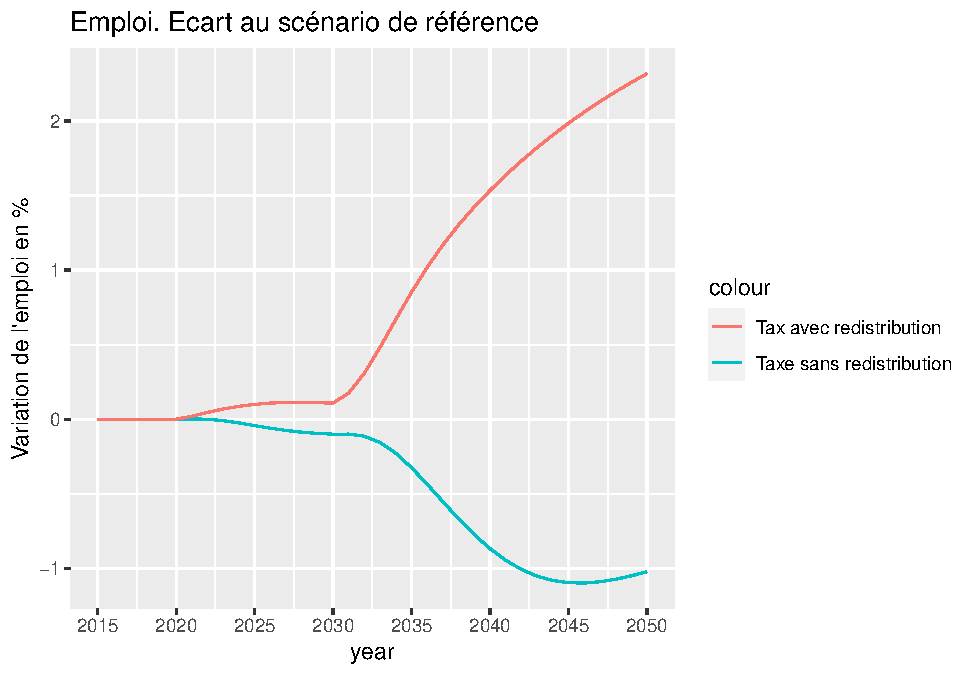
\includegraphics{Modele-ThreeMe-Tunisie_Sequeira_Valilou_Wang_files/figure-latex/unnamed-chunk-9-1.pdf}

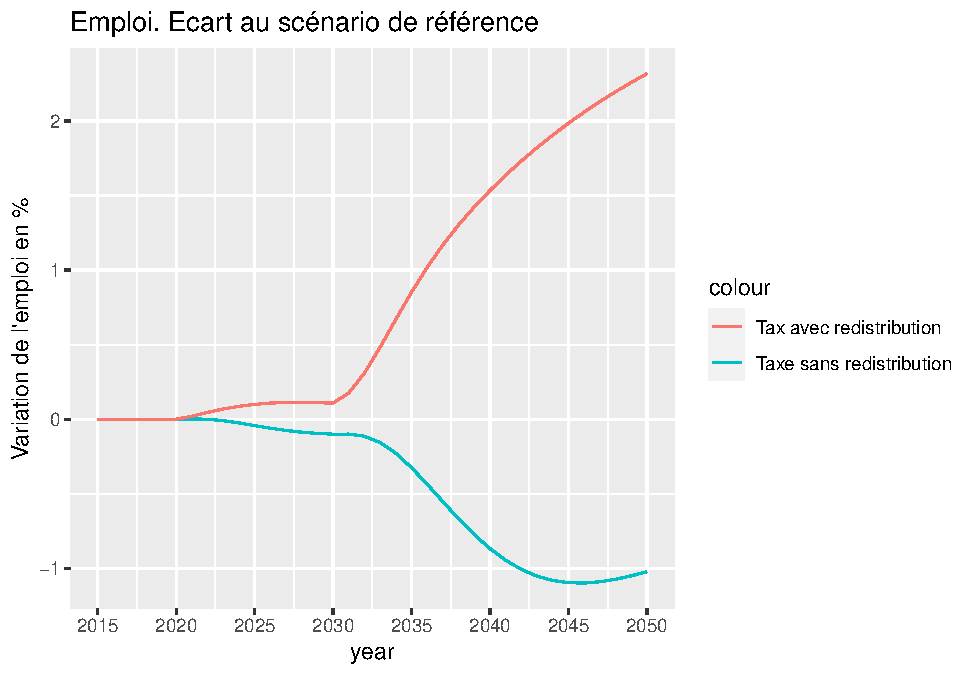
\includegraphics{Modele-ThreeMe-Tunisie_Sequeira_Valilou_Wang_files/figure-latex/unnamed-chunk-10-1.pdf}

Sectorial level analysis, Economy Structure: main sectors are
electricity (positive) and energy transformation (negative) what
happened in these two sectors? a developpement of electricity
production, and a recession of energy transformation

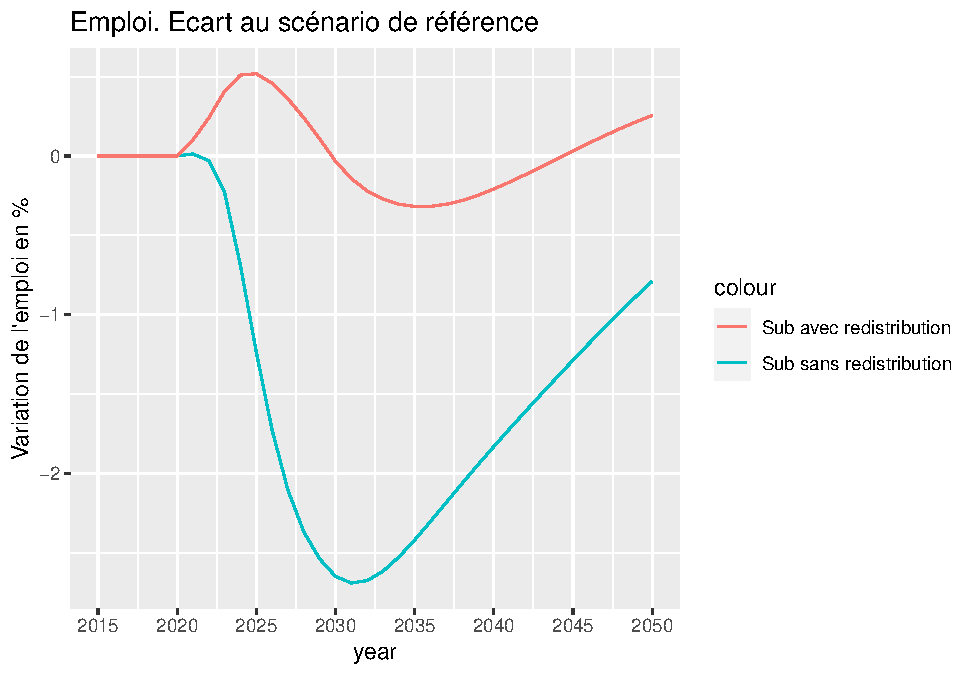
\includegraphics{Modele-ThreeMe-Tunisie_Sequeira_Valilou_Wang_files/figure-latex/unnamed-chunk-11-1.pdf}
\includegraphics{Modele-ThreeMe-Tunisie_Sequeira_Valilou_Wang_files/figure-latex/unnamed-chunk-11-2.pdf}

Energy intensity -\textgreater{} we observe the improvement of energy
efficiency, in another word the decrement of energy intensity, for all
the sectors of Tunisia's economy, especially for electricity and
industry \& agriculture. explained by the global drop of energy
consumption, coupled with the augmentation of added value in certain
sectors

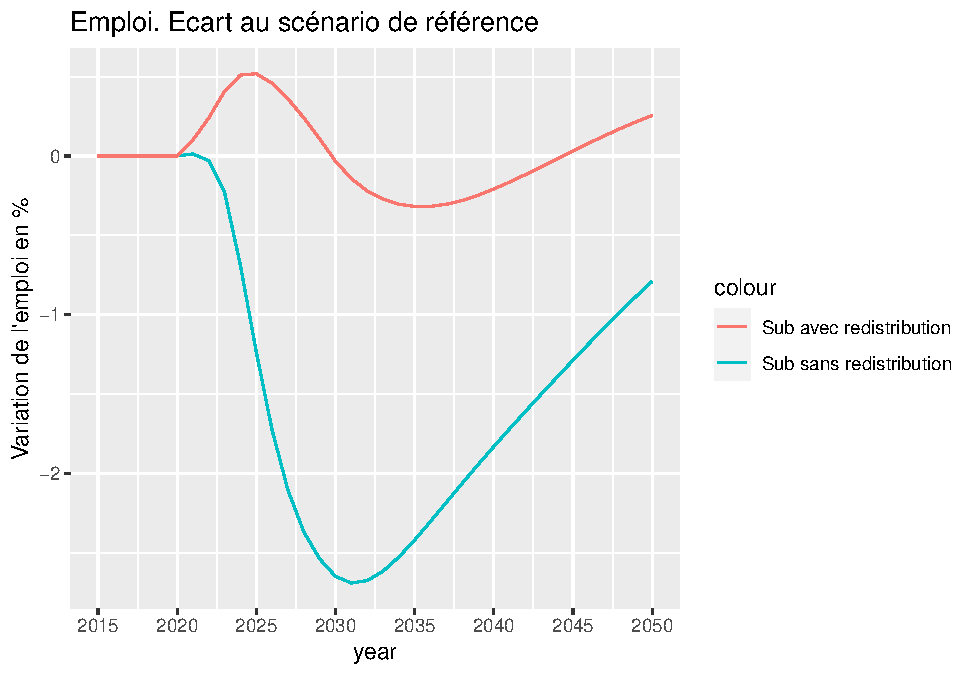
\includegraphics{Modele-ThreeMe-Tunisie_Sequeira_Valilou_Wang_files/figure-latex/unnamed-chunk-12-1.pdf}

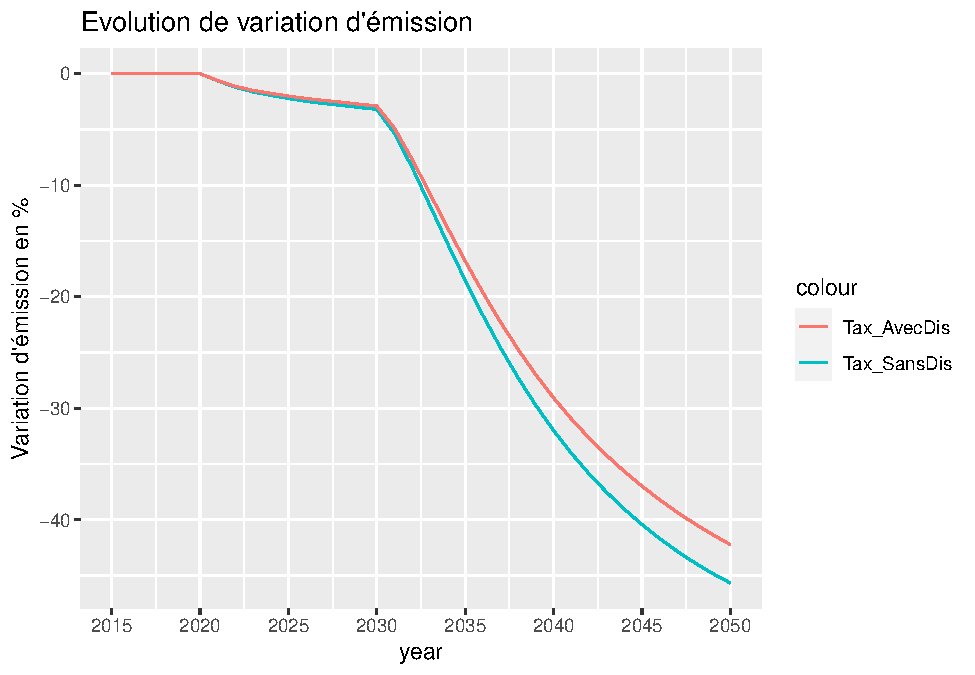
\includegraphics{Modele-ThreeMe-Tunisie_Sequeira_Valilou_Wang_files/figure-latex/unnamed-chunk-13-1.pdf}

Carbon intensity Dramastically change in energy transformation and
industry\&agriculture for energy transformation: -\textgreater{} explain
the integration of household into this sector -\textgreater{} mainly
from less consumption of fuels for transportation, and a increment of
electricity -\textgreater{} maybe because the electrical car or hybride
car. A slight reduction of natural gas consumption in energy
transformation for industry \& agriculture: same tendance, less natural
gas, less consumption of fuels for transportation, more electricity (for
transportation and heating etc)

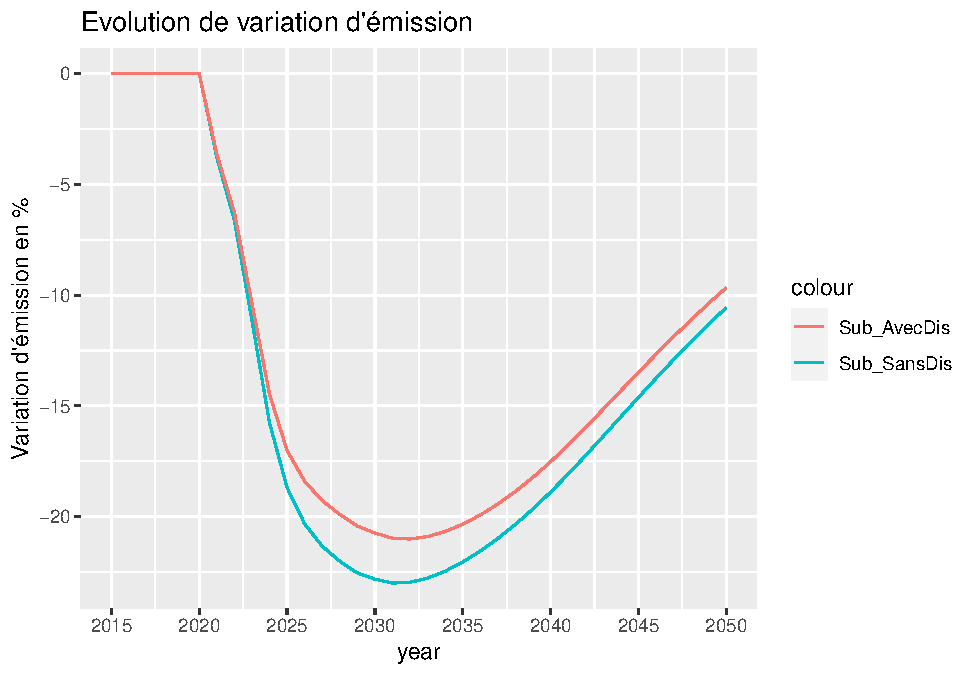
\includegraphics{Modele-ThreeMe-Tunisie_Sequeira_Valilou_Wang_files/figure-latex/unnamed-chunk-14-1.pdf}

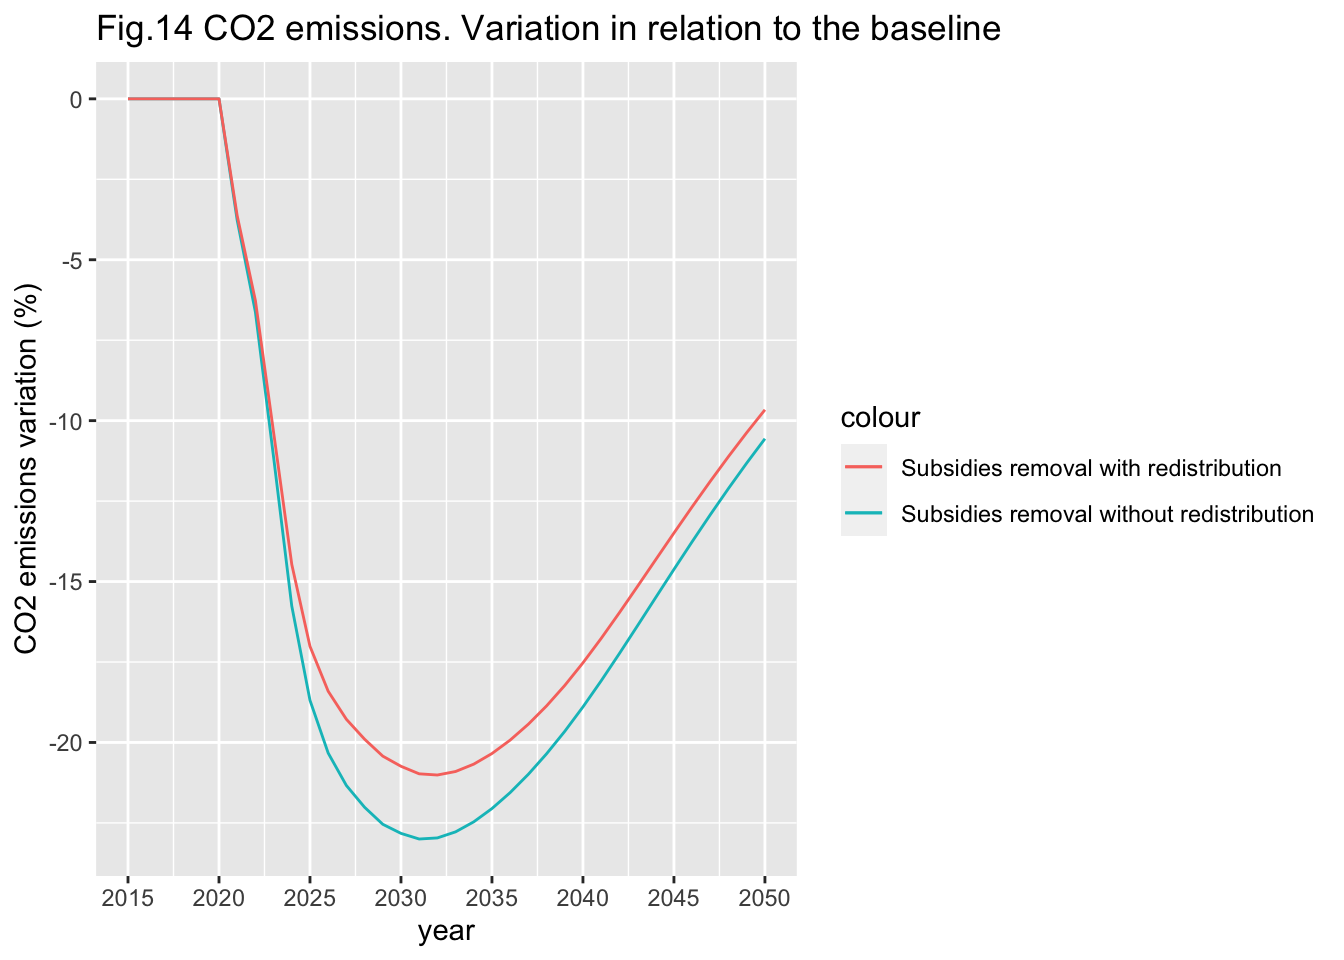
\includegraphics{Modele-ThreeMe-Tunisie_Sequeira_Valilou_Wang_files/figure-latex/unnamed-chunk-15-1.pdf}

For energy transformation, we creat a table, which is better than a
figure

\begin{longtabu} to \linewidth {>{\raggedright}X>{\raggedleft}X>{\raggedleft}X>{\raggedleft}X>{\raggedleft}X>{\raggedleft}X>{\raggedleft}X>{\raggedleft}X}
\caption{\label{tab:unnamed-chunk-16}Energy mix of sector Energy Transformation (in %) 
 for Carbon tax scenario and Baseline scenario}\\
\toprule
\textbf{ } & \textbf{2021} & \textbf{2025} & \textbf{2030} & \textbf{2035} & \textbf{2040} & \textbf{2045} & \textbf{2050}\\
\midrule
\endfirsthead
\caption[]{Energy mix of sector Energy Transformation (in  \textit{(continued)}}\\
\toprule
\textbf{ } & \textbf{2021} & \textbf{2025} & \textbf{2030} & \textbf{2035} & \textbf{2040} & \textbf{2045} & \textbf{2050}\\
\midrule
\endhead

\endfoot
\bottomrule
\endlastfoot
\addlinespace[0.3em]
\multicolumn{8}{l}{\textbf{Carbon Tax}}\\
\hspace{1em}\cellcolor{gray!6}{Crude oil} & \cellcolor{gray!6}{19.21} & \cellcolor{gray!6}{13.99} & \cellcolor{gray!6}{11.39} & \cellcolor{gray!6}{10.40} & \cellcolor{gray!6}{9.76} & \cellcolor{gray!6}{9.64} & \cellcolor{gray!6}{9.80}\\
\hspace{1em}Natural gas & 79.90 & 85.17 & 87.84 & 88.87 & 89.58 & 89.77 & 89.67\\
\hspace{1em}\cellcolor{gray!6}{Fuels for transportation} & \cellcolor{gray!6}{0.26} & \cellcolor{gray!6}{0.17} & \cellcolor{gray!6}{0.15} & \cellcolor{gray!6}{0.15} & \cellcolor{gray!6}{0.14} & \cellcolor{gray!6}{0.14} & \cellcolor{gray!6}{0.12}\\
\hspace{1em}Electricity & 0.63 & 0.66 & 0.63 & 0.58 & 0.51 & 0.45 & 0.41\\
\hspace{1em}\cellcolor{gray!6}{Fuels for other use} & \cellcolor{gray!6}{0.00} & \cellcolor{gray!6}{0.00} & \cellcolor{gray!6}{0.00} & \cellcolor{gray!6}{0.00} & \cellcolor{gray!6}{0.00} & \cellcolor{gray!6}{0.00} & \cellcolor{gray!6}{\vphantom{1} 0.00}\\
\addlinespace[0.3em]
\multicolumn{8}{l}{\textbf{Baseline}}\\
\hspace{1em}Crude oil & 19.20 & 13.88 & 11.25 & 9.66 & 8.11 & 7.25 & 6.78\\
\hspace{1em}\cellcolor{gray!6}{Natural gas} & \cellcolor{gray!6}{79.90} & \cellcolor{gray!6}{85.28} & \cellcolor{gray!6}{87.97} & \cellcolor{gray!6}{89.55} & \cellcolor{gray!6}{91.11} & \cellcolor{gray!6}{91.99} & \cellcolor{gray!6}{92.47}\\
\hspace{1em}Fuels for transportation & 0.27 & 0.17 & 0.15 & 0.16 & 0.17 & 0.18 & 0.18\\
\hspace{1em}\cellcolor{gray!6}{Electricity} & \cellcolor{gray!6}{0.63} & \cellcolor{gray!6}{0.66} & \cellcolor{gray!6}{0.63} & \cellcolor{gray!6}{0.62} & \cellcolor{gray!6}{0.60} & \cellcolor{gray!6}{0.58} & \cellcolor{gray!6}{0.56}\\
\hspace{1em}Fuels for other use & 0.00 & 0.00 & 0.00 & 0.00 & 0.00 & 0.00 & 0.00\\*
\end{longtabu}

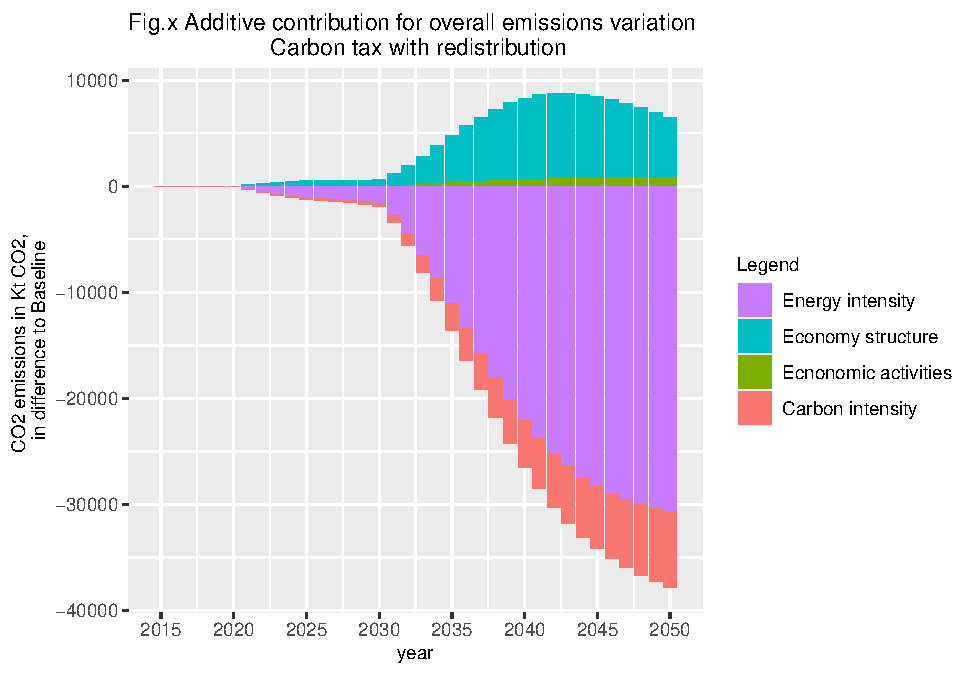
\includegraphics{Modele-ThreeMe-Tunisie_Sequeira_Valilou_Wang_files/figure-latex/unnamed-chunk-17-1.pdf}

Focus inter-sectoriel energy price will

1 - induce company to invest to reduce energy demande -\textgreater{}
une amelioration pour intensite energetique

2 - renwable energy -\textgreater{} une amelioration pour intensite
carbone, mais dans notre modele ca se voit pas a cause de l'hypothese du
modele

\hypertarget{lifting-of-energy-subsidies-bee}{%
\subsection{Lifting of energy subsidies
(bee)}\label{lifting-of-energy-subsidies-bee}}

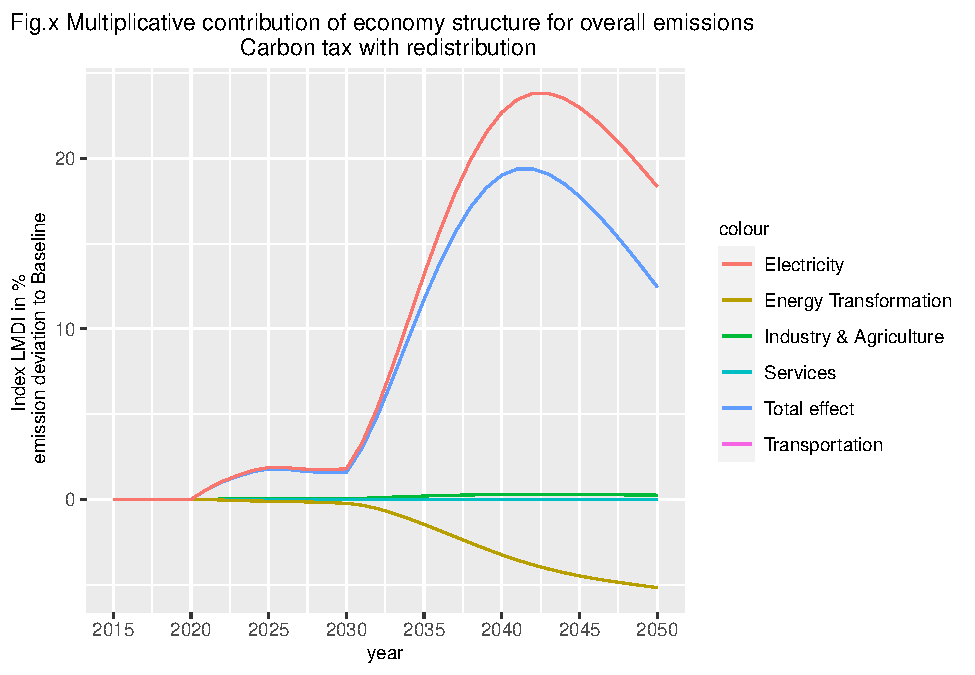
\includegraphics{Modele-ThreeMe-Tunisie_Sequeira_Valilou_Wang_files/figure-latex/unnamed-chunk-18-1.pdf}

\hypertarget{enr-1}{%
\subsection{ENR}\label{enr-1}}

\hypertarget{snbc-1}{%
\subsection{SNBC}\label{snbc-1}}

\hypertarget{prolongements}{%
\section{Prolongements}\label{prolongements}}

\hypertarget{dautres-leviers-pour-analyser-ouverture}{%
\subsection{D'autres leviers pour analyser
(ouverture)}\label{dautres-leviers-pour-analyser-ouverture}}

\hypertarget{lamuxe9lioration-du-cadre-statistique}{%
\subsection{L'amélioration du cadre
statistique}\label{lamuxe9lioration-du-cadre-statistique}}

OUverture : pb du secteur informel non pris en compte par la
comptabilité nationale

\hypertarget{conclusion}{%
\section{Conclusion}\label{conclusion}}

\printbibliography[title=Bibliographie]

\end{document}
